\begin{figure}
    \begin{center}
        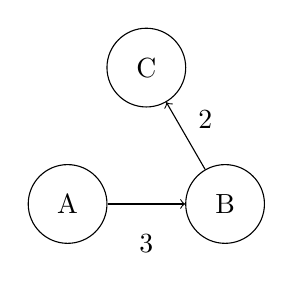
\begin{tikzpicture}            
            % Define vertices
            \node[circle,draw,minimum size=1cm] (A) at (0,0) {A};
            \node[circle,draw,minimum size=1cm] (B) at (2,0) {B};
            \node[circle,draw,minimum size=1cm] (C) at (1,1.732) {C};
            \node at (1, -0.5) {3};
            \node at (1.75, 1.075) {2};
            
            % Draw edges
            \draw[->](A) -- (B);
            \draw[->](B) -- (C);
            \end{tikzpicture}
        \caption{A simple attributed graph with three named vertices and two directed weighted edges.}
        \label{figure:graph-weighted}          
    \end{center}
\end{figure}